Para cumplir con uno de los primeros objetivos de este trabajo, se necesitaba
realizar una búsqueda de artículos científicos sobre esta temática:
\textit{Simulación de crecimiento de tumores con autómatas celulares}.

Tras una primera selección, donde se descartaron los artículos de \textit{arXiv}\footnote{\url{https://arxiv.org/}},
ya que, podrían estar aún en fase de revisión, así como, artículos demasiado antiguos o artículos
cuyo enfoque quedaran fuera del ámbito de la inteligencia artificial, se obtuvo una lista
con dos candidatos.

De los artículos seleccionados, se procedió a su estudio y extracción de información. A continuación,
se presenta la lista de trabajos obtenidos y, posteriormente, se describen los trabajos candidatos.

\section{Resultado de la búsqueda de artículos}

Los artículos encontrados durante la fase de búsqueda de información respecto a la temática
\textit{Simulación de crecimiento de tumores con autómatas celulares} son los siguientes:

\begin{itemize}
    \item \textit{Simulated Bain Tumor Growth Dynamics Using a Three-Dimensional Cellular Automaton}
    de A.R. Kansal, S. Torquato, G.R. Harsh IV, E.A. Chiocca and T.S. Deisboeck, 2000.
    \item \textit{A cellular automaton model for tumour growth in inhomogeneous environment}
    de T. Alarcon, H.M. Byrne, P.K. Maini, 2003.
    \item \textit{A Cellular automata model of tumor-immune system interactions}
    de D.G. Mallet, L.G. De Pillis, 2006.
    \item \textit{Cellular Automaton of Idealized Brain Tumor Growth Dynamics}
    de , 2009.
    \item \textit{A Review of Cellular Automata Models of tumor Growth}
    de Ankana Boondirek, Wannapong Triampo, Narin Nuttavut, 2010.
    \item \textit{Emergent Behaviors from A Cellular Automaton Model for Invasive Tumor Growth in Heterogeneous Microenvironments}
    de Yang Jiao, Salvatore Torquato, 2011-2012.
    \item \textit{Study of cancer hallmarks relevance using a cellular automaton tumor growth model}
    de José Santos, Ángel Monteagudo, 2012.
    \item \textit{Studying the capability of different cancer hallmarks to initiate tumor growth using a cellular automaton simulation. Application in a cancer stem cell context}
    de José Santos, Ángel Monteagudo, 2013.
    \item \textit{A Cellular Automaton Model for Tumor Dormancy: Emergence of a Proliferative Switch}
    de Duyu Chen, Yang Jiao, Salvatore Torquato, 2014.
    \item \textit{Analysis of behaviour transitions in tumor growth using a cellular automaton simulation}
    de José Santos, Ángel Monteagudo, 2014.
    \item \textit{Treatment analysis in a cancer stem cell context using a tumor growth model based on cellular automata}
    de José Santos, Ángel Monteagudo, 2015.
\end{itemize}

\section{\textit{Analysis of behaviour transitions in tumour growth
using a cellular automaton simulation}}

Este artículo \cite{jsantos-amonteagudo-1-2014} forma parte de una serie de artículos
\cite{jsantos-amonteagudo-2012} \cite{jsantos-amonteagudo-2013} \cite{jsantos-amonteagudo-2015}
en el cual los autores, con un enfoque genérico, pretenden simular el crecimiento de
tumores.

Para ello, se basan en varios trabajos, pero principalmente en los trabajos de Douglas Hanahan y Robert A. Weinberg
\cite{hanahan-weinberg-2000} \cite{hanahan-weinberg-2011}, donde se presentan varios marcadores presentes
en las células, los cuales consisten en una serie de mutaciones que permiten a las células presentar
un comportamiento canceroso.

En su enfoque, utilizan un autómata celular que sigue un modelo de eventos, esto es, porque los autores
necesitan, por un lado, simular las escalas de tiempo, y por otro, modelizar cuándo las células necesitan
realizar la mitosis.

En cada uno de sus trabajos, presentan diferentes enfoques. Esto es, se centran, o descartan, varios marcadores y
comportamientos. Por ejemplo, en el trabajo en el que se centra este proyecto \cite{jsantos-amonteagudo-1-2014}
los autores deciden ignorar dos marcadores, \textit{AG} o angiogénesis, y \textit{MT} o metástasis.

Además, deciden no modelizar el crecimiento celular, es decir, todas las células en la rejilla ocupan
el mismo espacio.

Es un enfoque genérico, que permite simular cualquier tipo de tumor modificando los parámetros de la
simulación, y permite también estudiar los distintos comportamientos emergentes según
qué marcador toma o no relevancia frente al resto.

\section{\textit{Cellular automaton of idealized brain tumor growth dynamics}}

Este artículo \cite{kansal-torquato} es uno de los dos candidatos estudiados con el objetivo
de desarrollar este proyecto.

En él, se presenta un nuevo modelo de autómata celular para simular crecimientos emergente de tumores cerebrales.
En concreto, se enfoca a un tipo de tumor, el tumor de Gompertzian. Los autores presentan
la consecución de simular el crecimiento de dicho tumor en casi tres órdenes de magnitud en radio
utilizando sólo cuatro parámetros microscópicos.

Su estudio tiene un elevado enfoque clínico modelizando la densidad de células y
el tamaño de cada célula, empleando el algoritmo de triangulación \textit{Delaunay}\footnote{\url{https://es.wikipedia.org/wiki/Triangulacion_de_Delaunay}}
junto a Polígonos de \textit{Thiessen} o diagramas de \textit{Voronoi}\footnote{\url{https://es.wikipedia.org/wiki/Poligonos_de_Thiessen}} para su representación.

\begin{figure}[h]
\centering
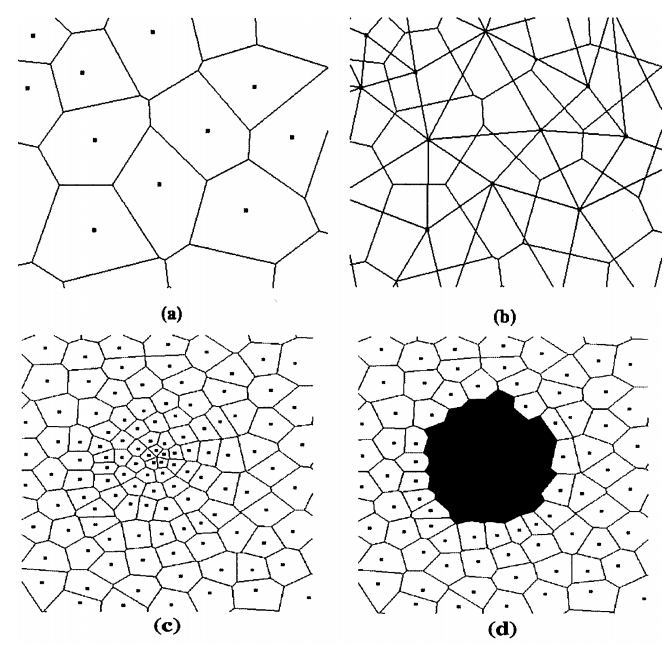
\includegraphics[scale=0.7]{figures/modelado_tamanio}
\caption{Triangulación de Delaunay junto a Polígonos de Thiessen o diagramas de Voronoi para modelizar el tamaño de las células.}
\end{figure}

Realizan también un modelado temporal, para así estudiar la velocidad de crecimiento de los tumores.
Sus resultados están muy especializados en un tipo de tumor, por lo que no realizan un estudio genérico
para varios tipos de tumores, con diferentes parámetros, configuraciones o marcadores.
